\Exhibit{BeaDigitalEconomy}{%
    New and Revised Statistics of the U.S. Digital Economy, 2005–2021, by \Bea, selected pages%
}

This report shows that:

\begin{itemize}

    \item \Quote{%
        Growth in price-adjusted GDP (also referred to as `chained-dollar' or `real'
        GDP) was \ul{9.8 percent} in 2021, \ul{greatly outpacing growth in the overall economy}, which increased 5.9 percent.%
    }

    \item \Quote{\dots software (12.1 percent)\dots experienced strong growth rates in 2021.}

    \item Software is responsible for \$722 billion of the total \$3.7 trillion gross output.

\end{itemize}

It is available at this address:\\
https://www.bea.gov/system/files/2022-11/new-and-revised-statistics-of-the-us-digital-economy-2005-2021.pdf

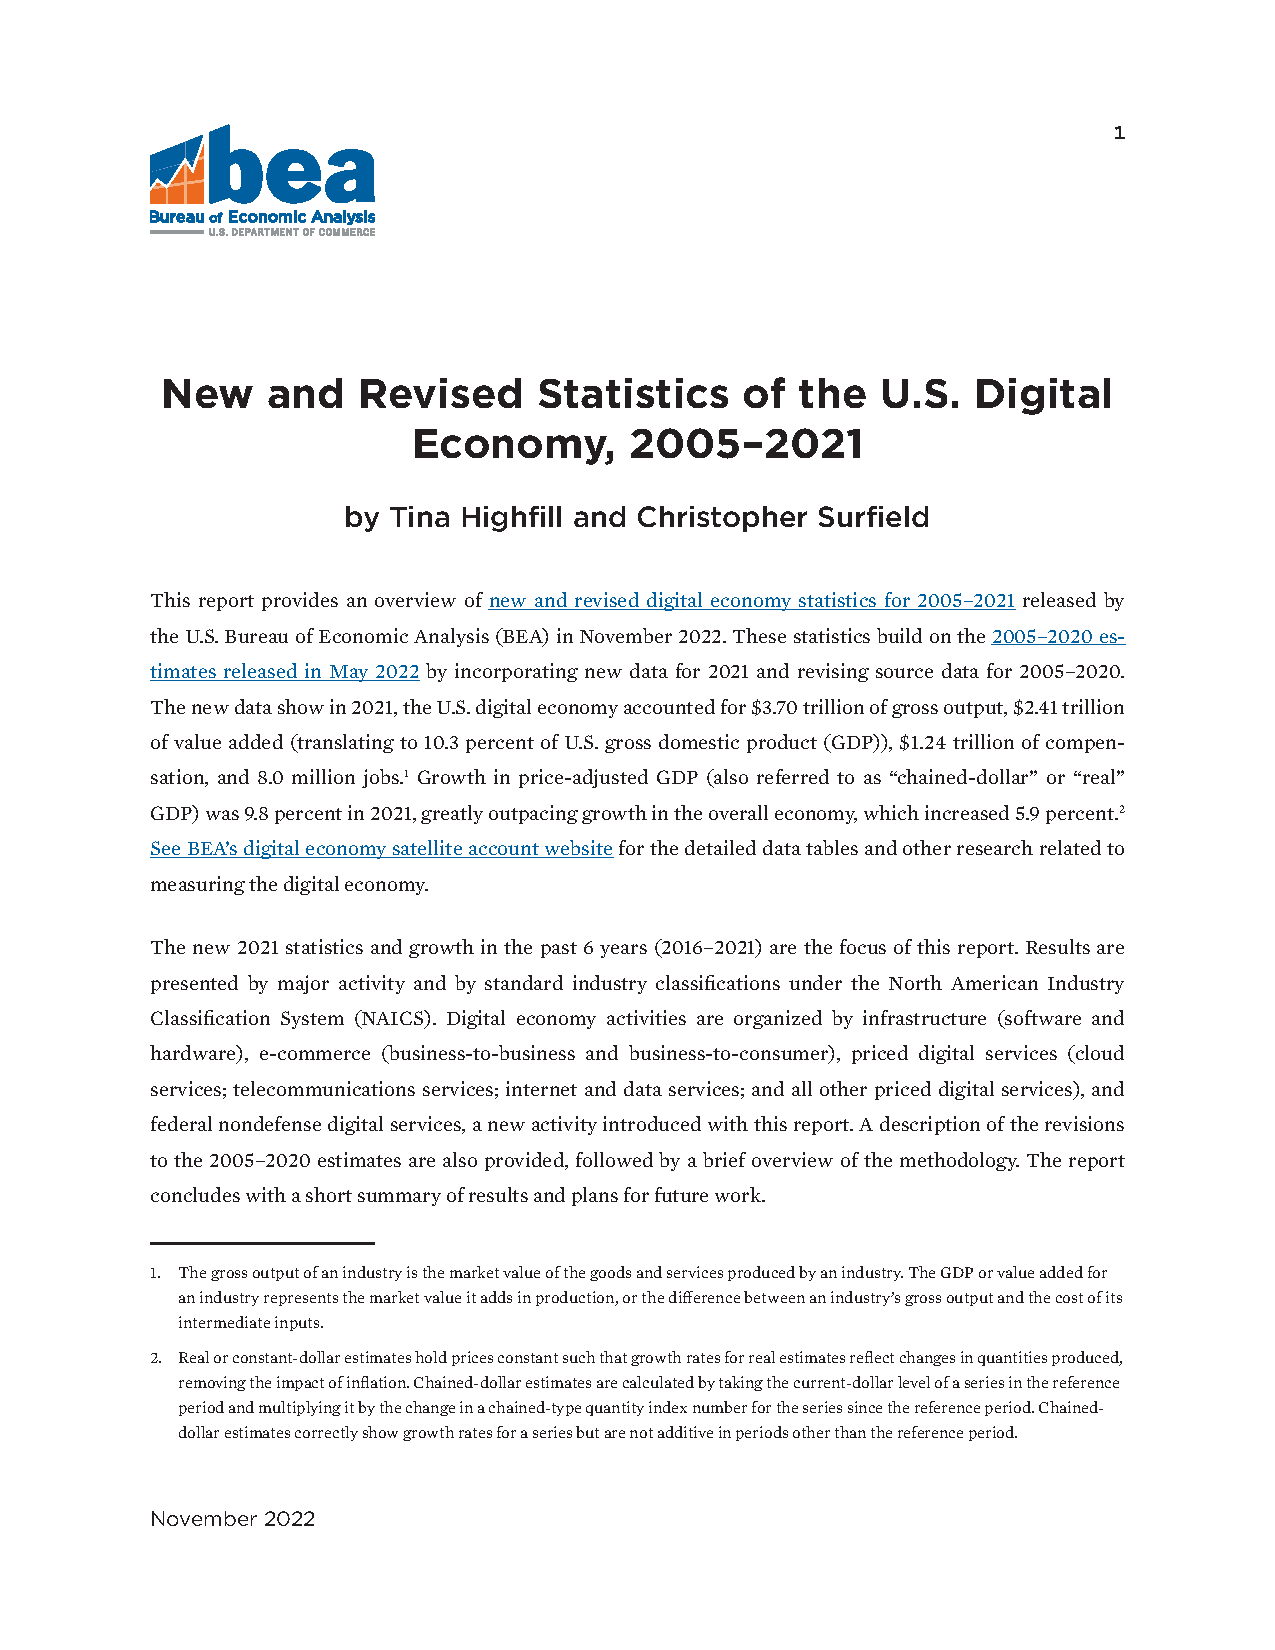
\includepdf[pages={1-3}]{new-and-revised-statistics-of-the-us-digital-economy-2005-2021}

\pagebreak
